\documentclass[11pt]{article}

    \usepackage[breakable]{tcolorbox}
    \usepackage{parskip} % Stop auto-indenting (to mimic markdown behaviour)
    

    % Basic figure setup, for now with no caption control since it's done
    % automatically by Pandoc (which extracts ![](path) syntax from Markdown).
    \usepackage{graphicx}
    % Keep aspect ratio if custom image width or height is specified
    \setkeys{Gin}{keepaspectratio}
    % Maintain compatibility with old templates. Remove in nbconvert 6.0
    \let\Oldincludegraphics\includegraphics
    % Ensure that by default, figures have no caption (until we provide a
    % proper Figure object with a Caption API and a way to capture that
    % in the conversion process - todo).
    \usepackage{caption}
    \DeclareCaptionFormat{nocaption}{}
    \captionsetup{format=nocaption,aboveskip=0pt,belowskip=0pt}

    \usepackage{float}
    \floatplacement{figure}{H} % forces figures to be placed at the correct location
    \usepackage{xcolor} % Allow colors to be defined
    \usepackage{enumerate} % Needed for markdown enumerations to work
    \usepackage{geometry} % Used to adjust the document margins
    \usepackage{amsmath} % Equations
    \usepackage{amssymb} % Equations
    \usepackage{textcomp} % defines textquotesingle
    % Hack from http://tex.stackexchange.com/a/47451/13684:
    \AtBeginDocument{%
        \def\PYZsq{\textquotesingle}% Upright quotes in Pygmentized code
    }
    \usepackage{upquote} % Upright quotes for verbatim code
    \usepackage{eurosym} % defines \euro
    \usepackage[ngerman]{babel}

    \usepackage{iftex}
    \ifPDFTeX
        \usepackage[T1]{fontenc}
        \IfFileExists{alphabeta.sty}{
              \usepackage{alphabeta}
          }{
              \usepackage[mathletters]{ucs}
              \usepackage[utf8x]{inputenc}
          }
    \else
        \usepackage{fontspec}
        \usepackage{unicode-math}
    \fi

    \usepackage{fancyvrb} % verbatim replacement that allows latex
    \usepackage{grffile} % extends the file name processing of package graphics
                         % to support a larger range
    \makeatletter % fix for old versions of grffile with XeLaTeX
    \@ifpackagelater{grffile}{2019/11/01}
    {
      % Do nothing on new versions
    }
    {
      \def\Gread@@xetex#1{%
        \IfFileExists{"\Gin@base".bb}%
        {\Gread@eps{\Gin@base.bb}}%
        {\Gread@@xetex@aux#1}%
      }
    }
    \makeatother
    \usepackage[Export]{adjustbox} % Used to constrain images to a maximum size
    \adjustboxset{max size={0.9\linewidth}{0.9\paperheight}}

    % The hyperref package gives us a pdf with properly built
    % internal navigation ('pdf bookmarks' for the table of contents,
    % internal cross-reference links, web links for URLs, etc.)
    \usepackage{hyperref}
    % The default LaTeX title has an obnoxious amount of whitespace. By default,
    % titling removes some of it. It also provides customization options.
    \usepackage{titling}
    \usepackage{longtable} % longtable support required by pandoc >1.10
    \usepackage{booktabs}  % table support for pandoc > 1.12.2
    \usepackage{array}     % table support for pandoc >= 2.11.3
    \usepackage{calc}      % table minipage width calculation for pandoc >= 2.11.1
    \usepackage[inline]{enumitem} % IRkernel/repr support (it uses the enumerate* environment)
    \usepackage[normalem]{ulem} % ulem is needed to support strikethroughs (\sout)
                                % normalem makes italics be italics, not underlines
    \usepackage{soul}      % strikethrough (\st) support for pandoc >= 3.0.0
    \usepackage{mathrsfs}
    

    
    % Colors for the hyperref package
    \definecolor{urlcolor}{rgb}{0,.145,.698}
    \definecolor{linkcolor}{rgb}{.71,0.21,0.01}
    \definecolor{citecolor}{rgb}{.12,.54,.11}

    % ANSI colors
    \definecolor{ansi-black}{HTML}{3E424D}
    \definecolor{ansi-black-intense}{HTML}{282C36}
    \definecolor{ansi-red}{HTML}{E75C58}
    \definecolor{ansi-red-intense}{HTML}{B22B31}
    \definecolor{ansi-green}{HTML}{00A250}
    \definecolor{ansi-green-intense}{HTML}{007427}
    \definecolor{ansi-yellow}{HTML}{DDB62B}
    \definecolor{ansi-yellow-intense}{HTML}{B27D12}
    \definecolor{ansi-blue}{HTML}{208FFB}
    \definecolor{ansi-blue-intense}{HTML}{0065CA}
    \definecolor{ansi-magenta}{HTML}{D160C4}
    \definecolor{ansi-magenta-intense}{HTML}{A03196}
    \definecolor{ansi-cyan}{HTML}{60C6C8}
    \definecolor{ansi-cyan-intense}{HTML}{258F8F}
    \definecolor{ansi-white}{HTML}{C5C1B4}
    \definecolor{ansi-white-intense}{HTML}{A1A6B2}
    \definecolor{ansi-default-inverse-fg}{HTML}{FFFFFF}
    \definecolor{ansi-default-inverse-bg}{HTML}{000000}

    % common color for the border for error outputs.
    \definecolor{outerrorbackground}{HTML}{FFDFDF}

    % commands and environments needed by pandoc snippets
    % extracted from the output of `pandoc -s`
    \providecommand{\tightlist}{%
      \setlength{\itemsep}{0pt}\setlength{\parskip}{0pt}}
    \DefineVerbatimEnvironment{Highlighting}{Verbatim}{commandchars=\\\{\}}
    % Add ',fontsize=\small' for more characters per line
    \newenvironment{Shaded}{}{}
    \newcommand{\KeywordTok}[1]{\textcolor[rgb]{0.00,0.44,0.13}{\textbf{{#1}}}}
    \newcommand{\DataTypeTok}[1]{\textcolor[rgb]{0.56,0.13,0.00}{{#1}}}
    \newcommand{\DecValTok}[1]{\textcolor[rgb]{0.25,0.63,0.44}{{#1}}}
    \newcommand{\BaseNTok}[1]{\textcolor[rgb]{0.25,0.63,0.44}{{#1}}}
    \newcommand{\FloatTok}[1]{\textcolor[rgb]{0.25,0.63,0.44}{{#1}}}
    \newcommand{\CharTok}[1]{\textcolor[rgb]{0.25,0.44,0.63}{{#1}}}
    \newcommand{\StringTok}[1]{\textcolor[rgb]{0.25,0.44,0.63}{{#1}}}
    \newcommand{\CommentTok}[1]{\textcolor[rgb]{0.38,0.63,0.69}{\textit{{#1}}}}
    \newcommand{\OtherTok}[1]{\textcolor[rgb]{0.00,0.44,0.13}{{#1}}}
    \newcommand{\AlertTok}[1]{\textcolor[rgb]{1.00,0.00,0.00}{\textbf{{#1}}}}
    \newcommand{\FunctionTok}[1]{\textcolor[rgb]{0.02,0.16,0.49}{{#1}}}
    \newcommand{\RegionMarkerTok}[1]{{#1}}
    \newcommand{\ErrorTok}[1]{\textcolor[rgb]{1.00,0.00,0.00}{\textbf{{#1}}}}
    \newcommand{\NormalTok}[1]{{#1}}

    % Additional commands for more recent versions of Pandoc
    \newcommand{\ConstantTok}[1]{\textcolor[rgb]{0.53,0.00,0.00}{{#1}}}
    \newcommand{\SpecialCharTok}[1]{\textcolor[rgb]{0.25,0.44,0.63}{{#1}}}
    \newcommand{\VerbatimStringTok}[1]{\textcolor[rgb]{0.25,0.44,0.63}{{#1}}}
    \newcommand{\SpecialStringTok}[1]{\textcolor[rgb]{0.73,0.40,0.53}{{#1}}}
    \newcommand{\ImportTok}[1]{{#1}}
    \newcommand{\DocumentationTok}[1]{\textcolor[rgb]{0.73,0.13,0.13}{\textit{{#1}}}}
    \newcommand{\AnnotationTok}[1]{\textcolor[rgb]{0.38,0.63,0.69}{\textbf{\textit{{#1}}}}}
    \newcommand{\CommentVarTok}[1]{\textcolor[rgb]{0.38,0.63,0.69}{\textbf{\textit{{#1}}}}}
    \newcommand{\VariableTok}[1]{\textcolor[rgb]{0.10,0.09,0.49}{{#1}}}
    \newcommand{\ControlFlowTok}[1]{\textcolor[rgb]{0.00,0.44,0.13}{\textbf{{#1}}}}
    \newcommand{\OperatorTok}[1]{\textcolor[rgb]{0.40,0.40,0.40}{{#1}}}
    \newcommand{\BuiltInTok}[1]{{#1}}
    \newcommand{\ExtensionTok}[1]{{#1}}
    \newcommand{\PreprocessorTok}[1]{\textcolor[rgb]{0.74,0.48,0.00}{{#1}}}
    \newcommand{\AttributeTok}[1]{\textcolor[rgb]{0.49,0.56,0.16}{{#1}}}
    \newcommand{\InformationTok}[1]{\textcolor[rgb]{0.38,0.63,0.69}{\textbf{\textit{{#1}}}}}
    \newcommand{\WarningTok}[1]{\textcolor[rgb]{0.38,0.63,0.69}{\textbf{\textit{{#1}}}}}


    % Define a nice break command that doesn't care if a line doesn't already
    % exist.
    \def\br{\hspace*{\fill} \\* }
    % Math Jax compatibility definitions
    \def\gt{>}
    \def\lt{<}
    \let\Oldtex\TeX
    \let\Oldlatex\LaTeX
    \renewcommand{\TeX}{\textrm{\Oldtex}}
    \renewcommand{\LaTeX}{\textrm{\Oldlatex}}
    % Document parameters
    % Document title
    
    
    
    
    
    
    
% Pygments definitions
\makeatletter
\def\PY@reset{\let\PY@it=\relax \let\PY@bf=\relax%
    \let\PY@ul=\relax \let\PY@tc=\relax%
    \let\PY@bc=\relax \let\PY@ff=\relax}
\def\PY@tok#1{\csname PY@tok@#1\endcsname}
\def\PY@toks#1+{\ifx\relax#1\empty\else%
    \PY@tok{#1}\expandafter\PY@toks\fi}
\def\PY@do#1{\PY@bc{\PY@tc{\PY@ul{%
    \PY@it{\PY@bf{\PY@ff{#1}}}}}}}
\def\PY#1#2{\PY@reset\PY@toks#1+\relax+\PY@do{#2}}

\@namedef{PY@tok@w}{\def\PY@tc##1{\textcolor[rgb]{0.73,0.73,0.73}{##1}}}
\@namedef{PY@tok@c}{\let\PY@it=\textit\def\PY@tc##1{\textcolor[rgb]{0.24,0.48,0.48}{##1}}}
\@namedef{PY@tok@cp}{\def\PY@tc##1{\textcolor[rgb]{0.61,0.40,0.00}{##1}}}
\@namedef{PY@tok@k}{\let\PY@bf=\textbf\def\PY@tc##1{\textcolor[rgb]{0.00,0.50,0.00}{##1}}}
\@namedef{PY@tok@kp}{\def\PY@tc##1{\textcolor[rgb]{0.00,0.50,0.00}{##1}}}
\@namedef{PY@tok@kt}{\def\PY@tc##1{\textcolor[rgb]{0.69,0.00,0.25}{##1}}}
\@namedef{PY@tok@o}{\def\PY@tc##1{\textcolor[rgb]{0.40,0.40,0.40}{##1}}}
\@namedef{PY@tok@ow}{\let\PY@bf=\textbf\def\PY@tc##1{\textcolor[rgb]{0.67,0.13,1.00}{##1}}}
\@namedef{PY@tok@nb}{\def\PY@tc##1{\textcolor[rgb]{0.00,0.50,0.00}{##1}}}
\@namedef{PY@tok@nf}{\def\PY@tc##1{\textcolor[rgb]{0.00,0.00,1.00}{##1}}}
\@namedef{PY@tok@nc}{\let\PY@bf=\textbf\def\PY@tc##1{\textcolor[rgb]{0.00,0.00,1.00}{##1}}}
\@namedef{PY@tok@nn}{\let\PY@bf=\textbf\def\PY@tc##1{\textcolor[rgb]{0.00,0.00,1.00}{##1}}}
\@namedef{PY@tok@ne}{\let\PY@bf=\textbf\def\PY@tc##1{\textcolor[rgb]{0.80,0.25,0.22}{##1}}}
\@namedef{PY@tok@nv}{\def\PY@tc##1{\textcolor[rgb]{0.10,0.09,0.49}{##1}}}
\@namedef{PY@tok@no}{\def\PY@tc##1{\textcolor[rgb]{0.53,0.00,0.00}{##1}}}
\@namedef{PY@tok@nl}{\def\PY@tc##1{\textcolor[rgb]{0.46,0.46,0.00}{##1}}}
\@namedef{PY@tok@ni}{\let\PY@bf=\textbf\def\PY@tc##1{\textcolor[rgb]{0.44,0.44,0.44}{##1}}}
\@namedef{PY@tok@na}{\def\PY@tc##1{\textcolor[rgb]{0.41,0.47,0.13}{##1}}}
\@namedef{PY@tok@nt}{\let\PY@bf=\textbf\def\PY@tc##1{\textcolor[rgb]{0.00,0.50,0.00}{##1}}}
\@namedef{PY@tok@nd}{\def\PY@tc##1{\textcolor[rgb]{0.67,0.13,1.00}{##1}}}
\@namedef{PY@tok@s}{\def\PY@tc##1{\textcolor[rgb]{0.73,0.13,0.13}{##1}}}
\@namedef{PY@tok@sd}{\let\PY@it=\textit\def\PY@tc##1{\textcolor[rgb]{0.73,0.13,0.13}{##1}}}
\@namedef{PY@tok@si}{\let\PY@bf=\textbf\def\PY@tc##1{\textcolor[rgb]{0.64,0.35,0.47}{##1}}}
\@namedef{PY@tok@se}{\let\PY@bf=\textbf\def\PY@tc##1{\textcolor[rgb]{0.67,0.36,0.12}{##1}}}
\@namedef{PY@tok@sr}{\def\PY@tc##1{\textcolor[rgb]{0.64,0.35,0.47}{##1}}}
\@namedef{PY@tok@ss}{\def\PY@tc##1{\textcolor[rgb]{0.10,0.09,0.49}{##1}}}
\@namedef{PY@tok@sx}{\def\PY@tc##1{\textcolor[rgb]{0.00,0.50,0.00}{##1}}}
\@namedef{PY@tok@m}{\def\PY@tc##1{\textcolor[rgb]{0.40,0.40,0.40}{##1}}}
\@namedef{PY@tok@gh}{\let\PY@bf=\textbf\def\PY@tc##1{\textcolor[rgb]{0.00,0.00,0.50}{##1}}}
\@namedef{PY@tok@gu}{\let\PY@bf=\textbf\def\PY@tc##1{\textcolor[rgb]{0.50,0.00,0.50}{##1}}}
\@namedef{PY@tok@gd}{\def\PY@tc##1{\textcolor[rgb]{0.63,0.00,0.00}{##1}}}
\@namedef{PY@tok@gi}{\def\PY@tc##1{\textcolor[rgb]{0.00,0.52,0.00}{##1}}}
\@namedef{PY@tok@gr}{\def\PY@tc##1{\textcolor[rgb]{0.89,0.00,0.00}{##1}}}
\@namedef{PY@tok@ge}{\let\PY@it=\textit}
\@namedef{PY@tok@gs}{\let\PY@bf=\textbf}
\@namedef{PY@tok@ges}{\let\PY@bf=\textbf\let\PY@it=\textit}
\@namedef{PY@tok@gp}{\let\PY@bf=\textbf\def\PY@tc##1{\textcolor[rgb]{0.00,0.00,0.50}{##1}}}
\@namedef{PY@tok@go}{\def\PY@tc##1{\textcolor[rgb]{0.44,0.44,0.44}{##1}}}
\@namedef{PY@tok@gt}{\def\PY@tc##1{\textcolor[rgb]{0.00,0.27,0.87}{##1}}}
\@namedef{PY@tok@err}{\def\PY@bc##1{{\setlength{\fboxsep}{\string -\fboxrule}\fcolorbox[rgb]{1.00,0.00,0.00}{1,1,1}{\strut ##1}}}}
\@namedef{PY@tok@kc}{\let\PY@bf=\textbf\def\PY@tc##1{\textcolor[rgb]{0.00,0.50,0.00}{##1}}}
\@namedef{PY@tok@kd}{\let\PY@bf=\textbf\def\PY@tc##1{\textcolor[rgb]{0.00,0.50,0.00}{##1}}}
\@namedef{PY@tok@kn}{\let\PY@bf=\textbf\def\PY@tc##1{\textcolor[rgb]{0.00,0.50,0.00}{##1}}}
\@namedef{PY@tok@kr}{\let\PY@bf=\textbf\def\PY@tc##1{\textcolor[rgb]{0.00,0.50,0.00}{##1}}}
\@namedef{PY@tok@bp}{\def\PY@tc##1{\textcolor[rgb]{0.00,0.50,0.00}{##1}}}
\@namedef{PY@tok@fm}{\def\PY@tc##1{\textcolor[rgb]{0.00,0.00,1.00}{##1}}}
\@namedef{PY@tok@vc}{\def\PY@tc##1{\textcolor[rgb]{0.10,0.09,0.49}{##1}}}
\@namedef{PY@tok@vg}{\def\PY@tc##1{\textcolor[rgb]{0.10,0.09,0.49}{##1}}}
\@namedef{PY@tok@vi}{\def\PY@tc##1{\textcolor[rgb]{0.10,0.09,0.49}{##1}}}
\@namedef{PY@tok@vm}{\def\PY@tc##1{\textcolor[rgb]{0.10,0.09,0.49}{##1}}}
\@namedef{PY@tok@sa}{\def\PY@tc##1{\textcolor[rgb]{0.73,0.13,0.13}{##1}}}
\@namedef{PY@tok@sb}{\def\PY@tc##1{\textcolor[rgb]{0.73,0.13,0.13}{##1}}}
\@namedef{PY@tok@sc}{\def\PY@tc##1{\textcolor[rgb]{0.73,0.13,0.13}{##1}}}
\@namedef{PY@tok@dl}{\def\PY@tc##1{\textcolor[rgb]{0.73,0.13,0.13}{##1}}}
\@namedef{PY@tok@s2}{\def\PY@tc##1{\textcolor[rgb]{0.73,0.13,0.13}{##1}}}
\@namedef{PY@tok@sh}{\def\PY@tc##1{\textcolor[rgb]{0.73,0.13,0.13}{##1}}}
\@namedef{PY@tok@s1}{\def\PY@tc##1{\textcolor[rgb]{0.73,0.13,0.13}{##1}}}
\@namedef{PY@tok@mb}{\def\PY@tc##1{\textcolor[rgb]{0.40,0.40,0.40}{##1}}}
\@namedef{PY@tok@mf}{\def\PY@tc##1{\textcolor[rgb]{0.40,0.40,0.40}{##1}}}
\@namedef{PY@tok@mh}{\def\PY@tc##1{\textcolor[rgb]{0.40,0.40,0.40}{##1}}}
\@namedef{PY@tok@mi}{\def\PY@tc##1{\textcolor[rgb]{0.40,0.40,0.40}{##1}}}
\@namedef{PY@tok@il}{\def\PY@tc##1{\textcolor[rgb]{0.40,0.40,0.40}{##1}}}
\@namedef{PY@tok@mo}{\def\PY@tc##1{\textcolor[rgb]{0.40,0.40,0.40}{##1}}}
\@namedef{PY@tok@ch}{\let\PY@it=\textit\def\PY@tc##1{\textcolor[rgb]{0.24,0.48,0.48}{##1}}}
\@namedef{PY@tok@cm}{\let\PY@it=\textit\def\PY@tc##1{\textcolor[rgb]{0.24,0.48,0.48}{##1}}}
\@namedef{PY@tok@cpf}{\let\PY@it=\textit\def\PY@tc##1{\textcolor[rgb]{0.24,0.48,0.48}{##1}}}
\@namedef{PY@tok@c1}{\let\PY@it=\textit\def\PY@tc##1{\textcolor[rgb]{0.24,0.48,0.48}{##1}}}
\@namedef{PY@tok@cs}{\let\PY@it=\textit\def\PY@tc##1{\textcolor[rgb]{0.24,0.48,0.48}{##1}}}

\def\PYZbs{\char`\\}
\def\PYZus{\char`\_}
\def\PYZob{\char`\{}
\def\PYZcb{\char`\}}
\def\PYZca{\char`\^}
\def\PYZam{\char`\&}
\def\PYZlt{\char`\<}
\def\PYZgt{\char`\>}
\def\PYZsh{\char`\#}
\def\PYZpc{\char`\%}
\def\PYZdl{\char`\$}
\def\PYZhy{\char`\-}
\def\PYZsq{\char`\'}
\def\PYZdq{\char`\"}
\def\PYZti{\char`\~}
% for compatibility with earlier versions
\def\PYZat{@}
\def\PYZlb{[}
\def\PYZrb{]}
\makeatother


% For linebreaks inside Verbatim environment from package fancyvrb.
\makeatletter
    \newbox\Wrappedcontinuationbox
    \newbox\Wrappedvisiblespacebox
    \newcommand*\Wrappedvisiblespace {\textcolor{red}{\textvisiblespace}}
    \newcommand*\Wrappedcontinuationsymbol {\textcolor{red}{\llap{\tiny$\m@th\hookrightarrow$}}}
    \newcommand*\Wrappedcontinuationindent {3ex }
    \newcommand*\Wrappedafterbreak {\kern\Wrappedcontinuationindent\copy\Wrappedcontinuationbox}
    % Take advantage of the already applied Pygments mark-up to insert
    % potential linebreaks for TeX processing.
    %        {, <, #, %, $, ' and ": go to next line.
    %        _, }, ^, &, >, - and ~: stay at end of broken line.
    % Use of \textquotesingle for straight quote.
    \newcommand*\Wrappedbreaksatspecials {%
        \def\PYGZus{\discretionary{\char`\_}{\Wrappedafterbreak}{\char`\_}}%
        \def\PYGZob{\discretionary{}{\Wrappedafterbreak\char`\{}{\char`\{}}%
        \def\PYGZcb{\discretionary{\char`\}}{\Wrappedafterbreak}{\char`\}}}%
        \def\PYGZca{\discretionary{\char`\^}{\Wrappedafterbreak}{\char`\^}}%
        \def\PYGZam{\discretionary{\char`\&}{\Wrappedafterbreak}{\char`\&}}%
        \def\PYGZlt{\discretionary{}{\Wrappedafterbreak\char`\<}{\char`\<}}%
        \def\PYGZgt{\discretionary{\char`\>}{\Wrappedafterbreak}{\char`\>}}%
        \def\PYGZsh{\discretionary{}{\Wrappedafterbreak\char`\#}{\char`\#}}%
        \def\PYGZpc{\discretionary{}{\Wrappedafterbreak\char`\%}{\char`\%}}%
        \def\PYGZdl{\discretionary{}{\Wrappedafterbreak\char`\$}{\char`\$}}%
        \def\PYGZhy{\discretionary{\char`\-}{\Wrappedafterbreak}{\char`\-}}%
        \def\PYGZsq{\discretionary{}{\Wrappedafterbreak\textquotesingle}{\textquotesingle}}%
        \def\PYGZdq{\discretionary{}{\Wrappedafterbreak\char`\"}{\char`\"}}%
        \def\PYGZti{\discretionary{\char`\~}{\Wrappedafterbreak}{\char`\~}}%
    }
    % Some characters . , ; ? ! / are not pygmentized.
    % This macro makes them "active" and they will insert potential linebreaks
    \newcommand*\Wrappedbreaksatpunct {%
        \lccode`\~`\.\lowercase{\def~}{\discretionary{\hbox{\char`\.}}{\Wrappedafterbreak}{\hbox{\char`\.}}}%
        \lccode`\~`\,\lowercase{\def~}{\discretionary{\hbox{\char`\,}}{\Wrappedafterbreak}{\hbox{\char`\,}}}%
        \lccode`\~`\;\lowercase{\def~}{\discretionary{\hbox{\char`\;}}{\Wrappedafterbreak}{\hbox{\char`\;}}}%
        \lccode`\~`\:\lowercase{\def~}{\discretionary{\hbox{\char`\:}}{\Wrappedafterbreak}{\hbox{\char`\:}}}%
        \lccode`\~`\?\lowercase{\def~}{\discretionary{\hbox{\char`\?}}{\Wrappedafterbreak}{\hbox{\char`\?}}}%
        \lccode`\~`\!\lowercase{\def~}{\discretionary{\hbox{\char`\!}}{\Wrappedafterbreak}{\hbox{\char`\!}}}%
        \lccode`\~`\/\lowercase{\def~}{\discretionary{\hbox{\char`\/}}{\Wrappedafterbreak}{\hbox{\char`\/}}}%
        \catcode`\.\active
        \catcode`\,\active
        \catcode`\;\active
        \catcode`\:\active
        \catcode`\?\active
        \catcode`\!\active
        \catcode`\/\active
        \lccode`\~`\~
    }
\makeatother

\let\OriginalVerbatim=\Verbatim
\makeatletter
\renewcommand{\Verbatim}[1][1]{%
    %\parskip\z@skip
    \sbox\Wrappedcontinuationbox {\Wrappedcontinuationsymbol}%
    \sbox\Wrappedvisiblespacebox {\FV@SetupFont\Wrappedvisiblespace}%
    \def\FancyVerbFormatLine ##1{\hsize\linewidth
        \vtop{\raggedright\hyphenpenalty\z@\exhyphenpenalty\z@
            \doublehyphendemerits\z@\finalhyphendemerits\z@
            \strut ##1\strut}%
    }%
    % If the linebreak is at a space, the latter will be displayed as visible
    % space at end of first line, and a continuation symbol starts next line.
    % Stretch/shrink are however usually zero for typewriter font.
    \def\FV@Space {%
        \nobreak\hskip\z@ plus\fontdimen3\font minus\fontdimen4\font
        \discretionary{\copy\Wrappedvisiblespacebox}{\Wrappedafterbreak}
        {\kern\fontdimen2\font}%
    }%

    % Allow breaks at special characters using \PYG... macros.
    \Wrappedbreaksatspecials
    % Breaks at punctuation characters . , ; ? ! and / need catcode=\active
    \OriginalVerbatim[#1,codes*=\Wrappedbreaksatpunct]%
}
\makeatother

% Exact colors from NB
\definecolor{incolor}{HTML}{303F9F}
\definecolor{outcolor}{HTML}{D84315}
\definecolor{cellborder}{HTML}{CFCFCF}
\definecolor{cellbackground}{HTML}{F7F7F7}

% prompt
\makeatletter
\newcommand{\boxspacing}{\kern\kvtcb@left@rule\kern\kvtcb@boxsep}
\makeatother
\newcommand{\prompt}[4]{
    {\ttfamily\llap{{\color{#2}[#3]:\hspace{3pt}#4}}\vspace{-\baselineskip}}
}
    

    
% Prevent overflowing lines due to hard-to-break entities
\sloppy
% Setup hyperref package
\hypersetup{
  breaklinks=true,  % so long urls are correctly broken across lines
  colorlinks=true,
  urlcolor=urlcolor,
  linkcolor=linkcolor,
  citecolor=citecolor,
  }
% Slightly bigger margins than the latex defaults

\geometry{verbose,tmargin=1in,bmargin=1in,lmargin=1in,rmargin=1in}

\author{Gruppe 1: Marlene, Luca, Yassin}
\title{Laborbuch: Verhalten dehnbarer Stoffe}
    


\begin{document}
    
    \maketitle
    \date{}
    \tableofcontents
    \newpage

    \textbf{Ziel:}\label{ziel}
    Unser Ziel ist es das Verhalten dehnbarer Stoffe zu untersuchen und uns
    mit selbst entwickelten Experimenten zu beschäftigen.

    \section{Versuchsdurchführung Teil 1}\label{versuchsdurchfuxfchrung-teil-1}

    \subsection{Einleitung:}\label{einleitung}
    In unserem ersten Versuch wollen wir testen, ob das Hooksche Modell das
    Verhalten einiger zufällig ausgewählten dehnbaren Stoffen gut
    beschreibt.

    \subsection{Material:}
    \noindent\begin{minipage}{0.6\textwidth}\raggedright
    - Haargummi\\
    - verschiedene Gewichte von 25g bis 200g\\
    - Lineal\\
    - Haken\\
    - Metallstäbe\\
    - Schraubstock\\
    \end{minipage}%
    \hfill%
    \begin{minipage}{0.3\textwidth}
    \centering
    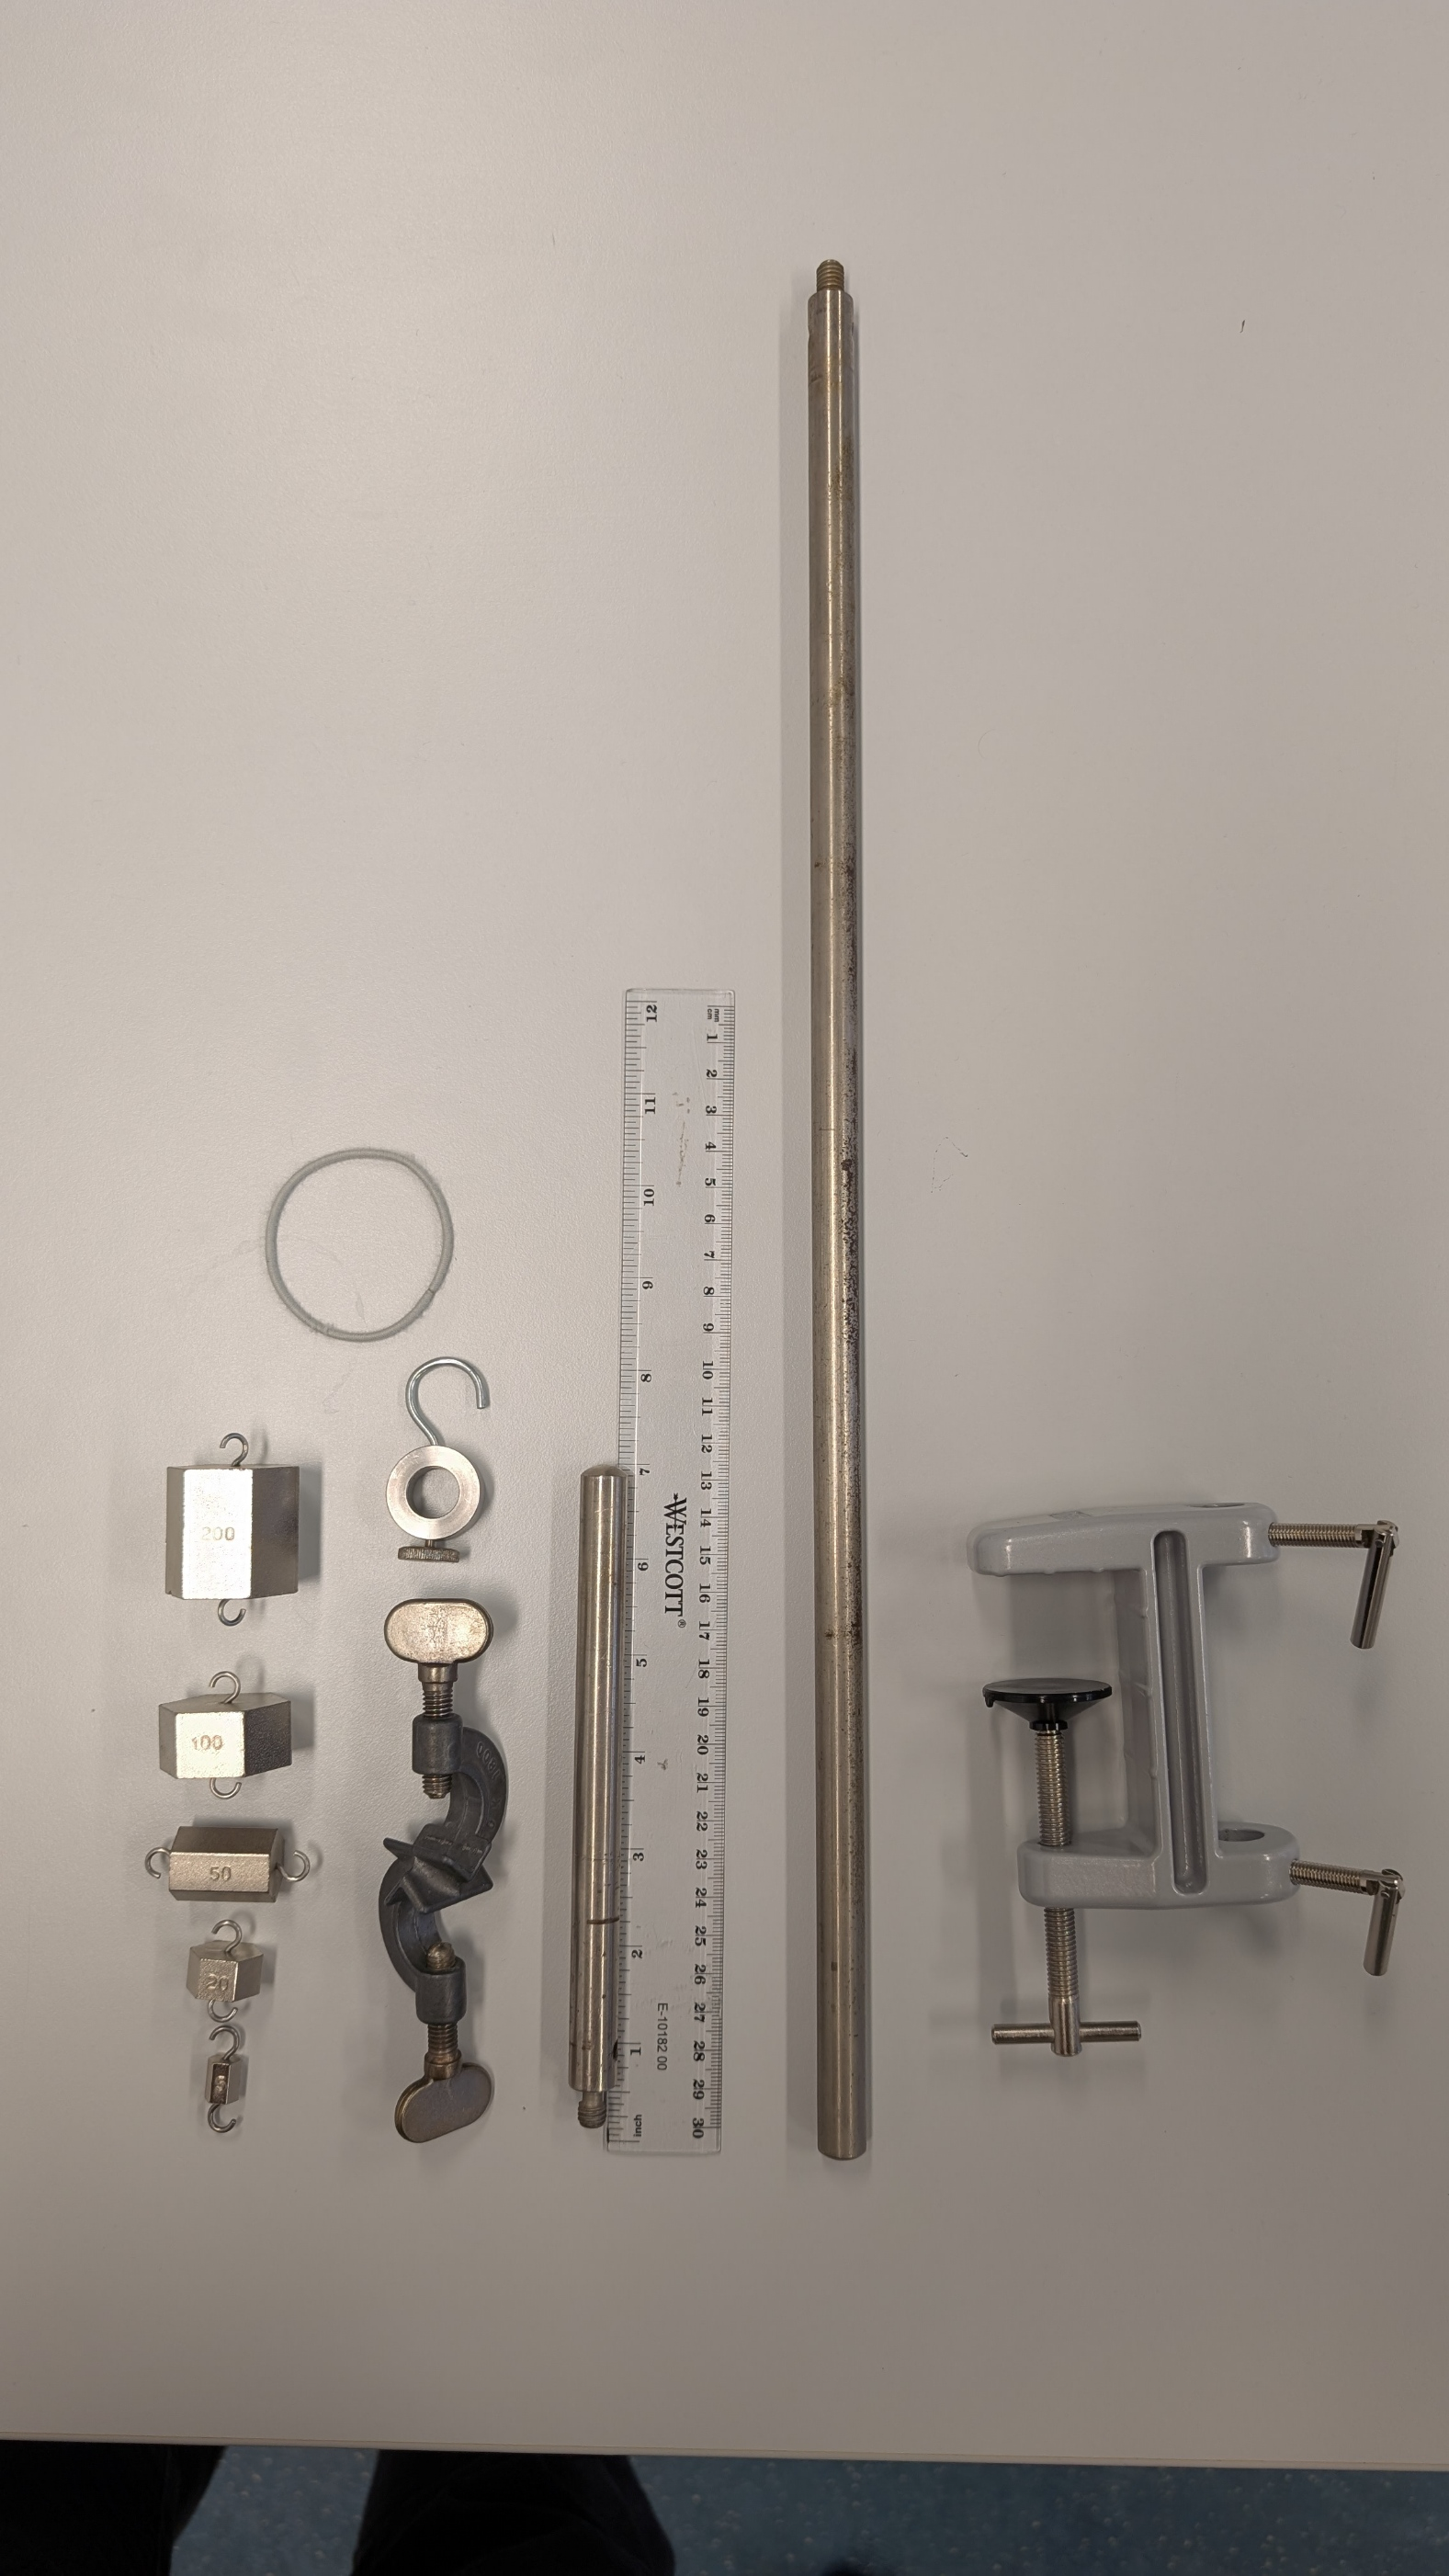
\includegraphics[width=0.95\linewidth]{PXL_20250107_141138099.jpg}
    \vspace{0.5em} % Abstand zwischen Bild und Unterschrift
    \textbf{Abbildung 1:} Beispiel einer Vorrichtung. % Manuelle Unterschrift
    \end{minipage}

    \subsection{Durchführung:}
    Messung der Auslenkung verschiedener Gewichte an einem Haargummi zur
    Bestimmung der Federkonstante.

    \subsection{Messgerät:}
    Das Lineal von Westcott. Es hat eine Ableseskala von 1mm und eine
    unbekannte Geräteunsicherheit, welche vermutlich vernachlässigbar ist.
    Die Messunsicherheit beträgt somit:\\
    \[
    u_x = \frac{u_{\text{Skala}}}{2*\sqrt{6}} = \frac{1 \, \text{mm}}{2*\sqrt{6}} \approx 0,20 \, \text{mm}
    \]

    \subsection{Versuchsaufbau:}
    \begin{center}
    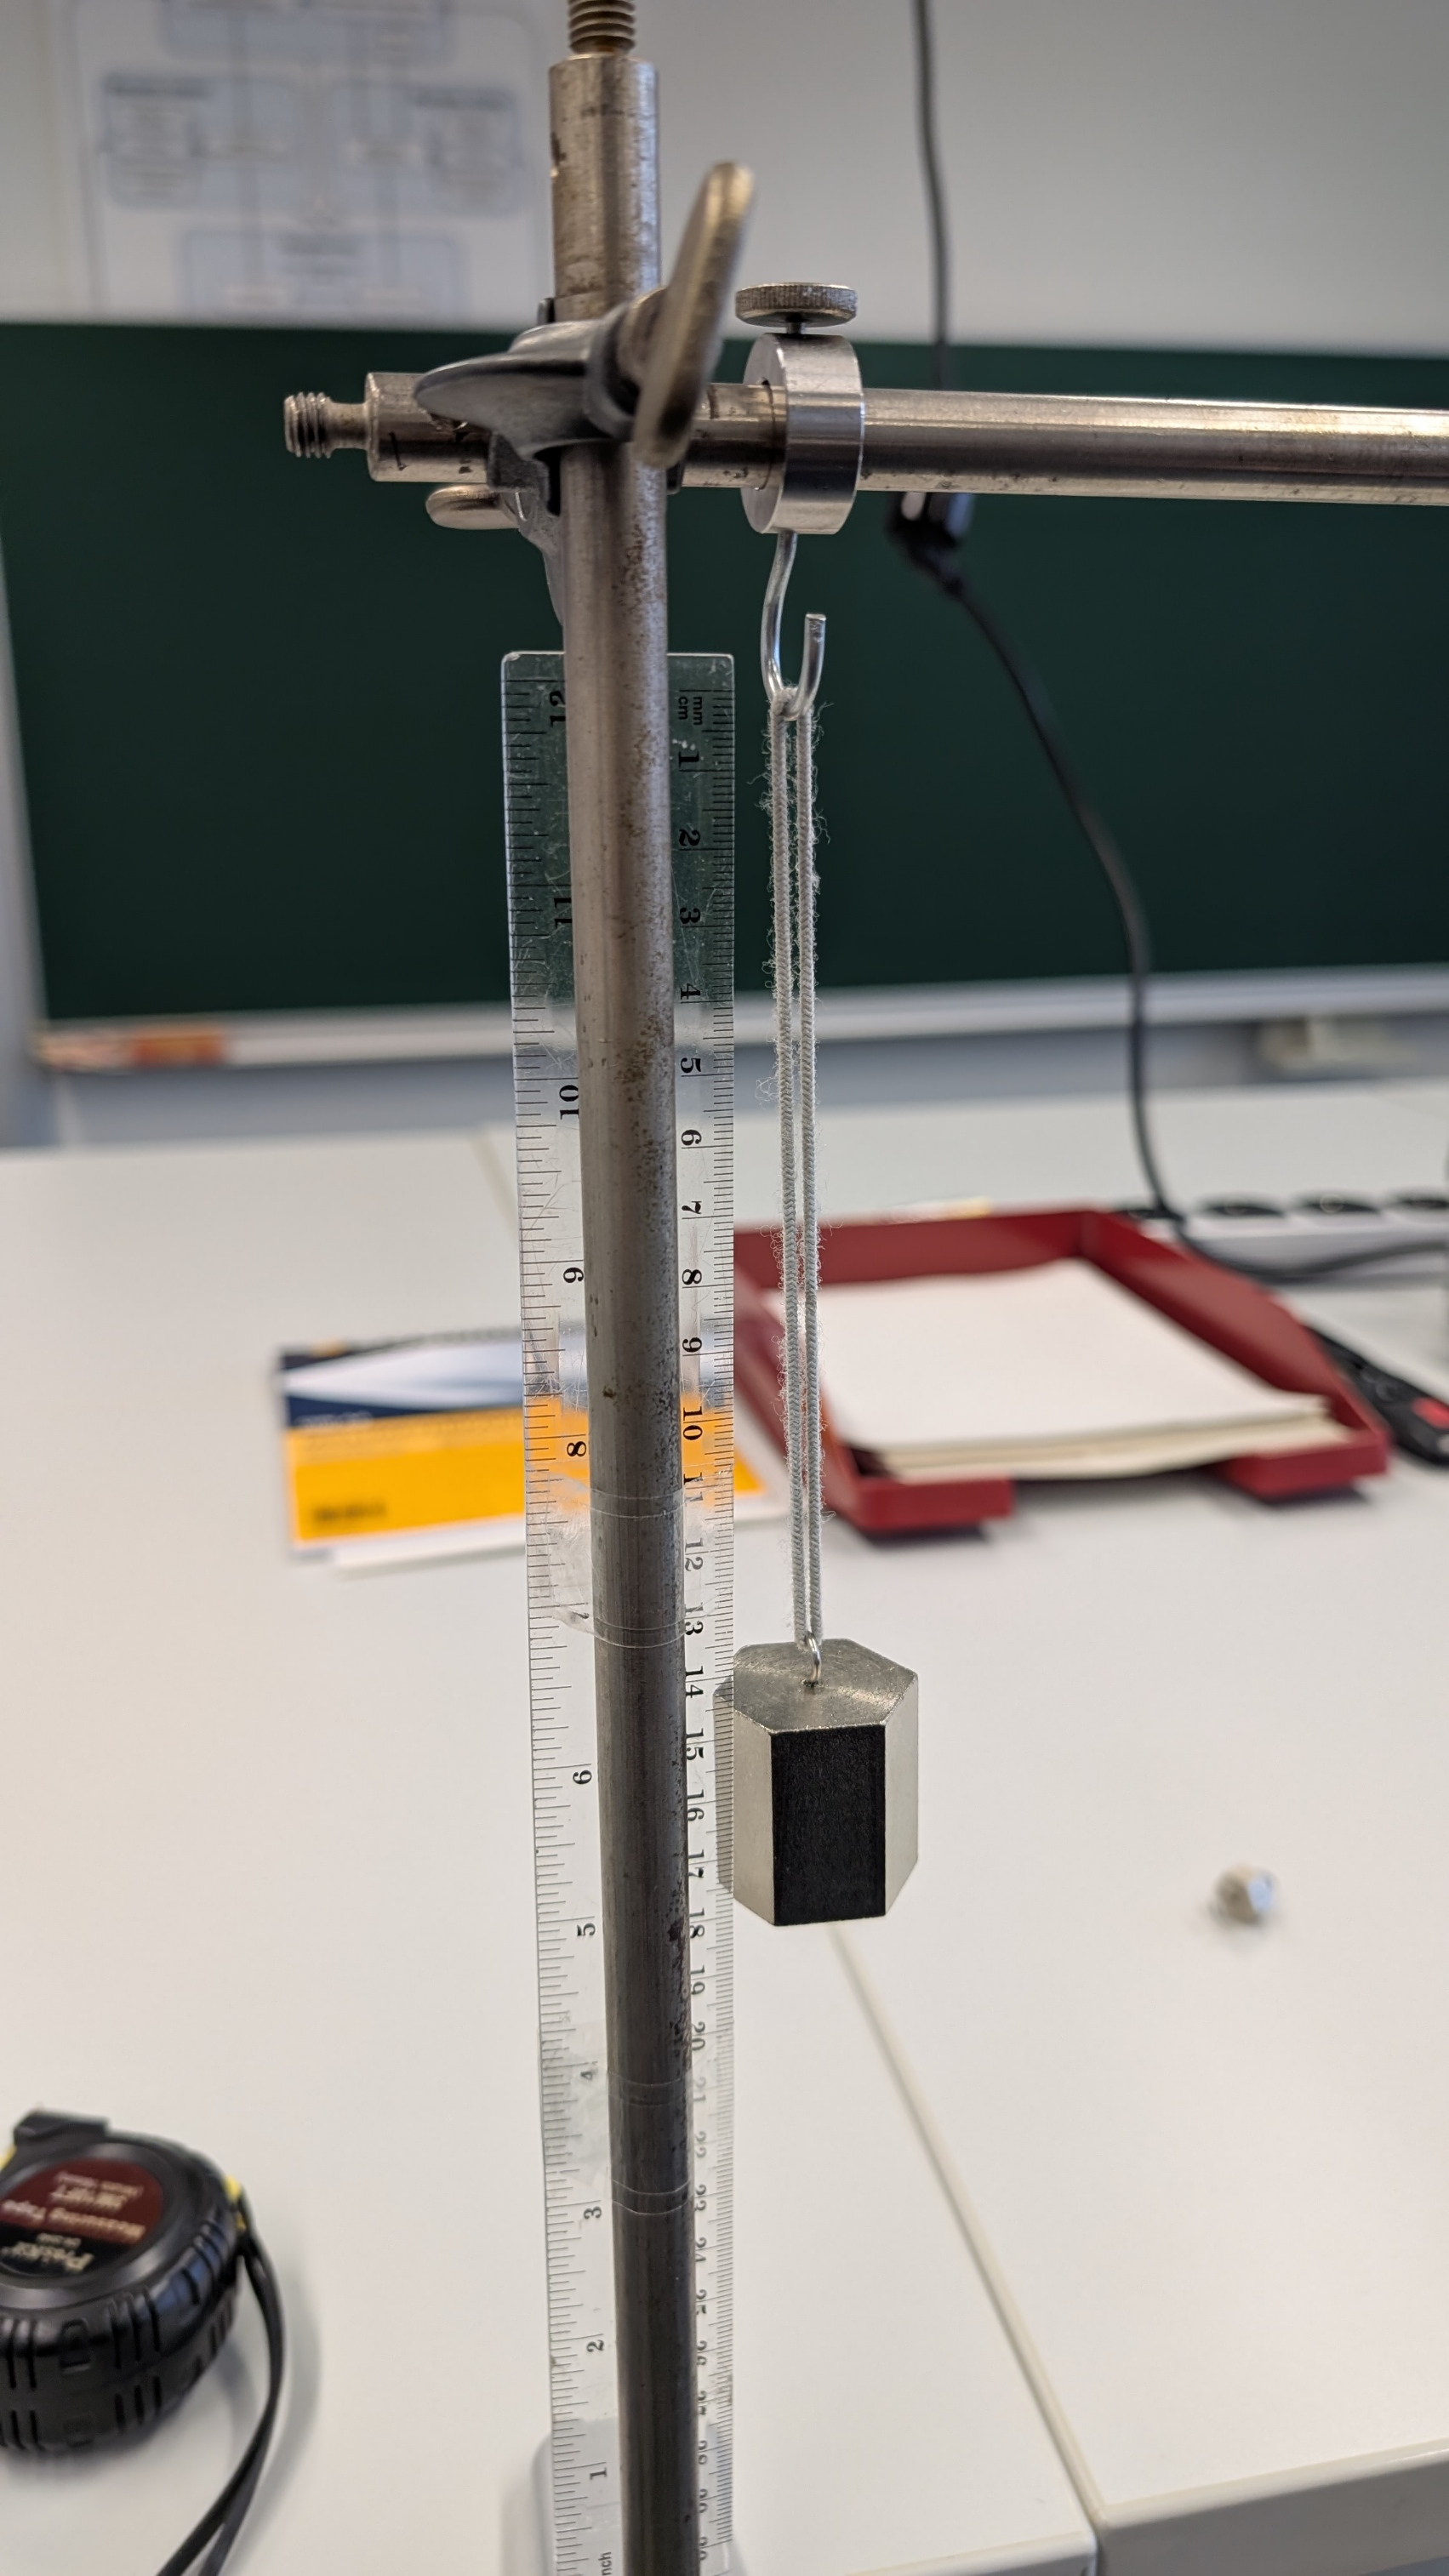
\includegraphics[width=0.29\textwidth]{PXL_20250107_114120921.jpg} \\
    \textbf{Abbildung 2:} Zusammengebaute Vorrichtung auf der man Gewichte ans Haargummi hängen kann um die Auslenkung zu messen.
    \end{center}
    
    
    \subsection{Messung:}\\
    \begin{longtable}[]{@{}ll@{}}
    \toprule\noalign{}
    Masse (g) & Messwert (mm) \\
    \midrule\noalign{}
    \endhead
    \bottomrule\noalign{}
    \endlastfoot
    0 & 56 \\
    25 & 75 \\
    50 & 80 \\
    100 & 91 \\
    150 & 117 \\
    200 & 142 \\
    250 & 158 \\
    300 & 165 \\
    350 & 171 \\
    400 & 173 \\
    \end{longtable}

    \subsection{Überlegungen:}\\
    Beim Ablesen ist uns aufgefallen, dass es teilweise schwer war
    herauszufinden wie weit unten die Gewichte sind, da sie nicht direkt
    neben dem Lineal standen und dadurch sich Ableseparallaxe gebildet
    haben.\\
    
    Außerdem haben wir festgestellt, dass die Gewichte möglicherweise durch
    Abnutzung, falsche Normung nicht korrekt sind und haben deswegen nochmal
    nachgemessen.
    
    \subsection{Messgerät 2:}\\
    Die Waage EK-6000H von A\&D Instruments .Es hat eine Ableseskala von
    0,1g und eine Geräteunsicherheit von 0,1g. Die Messunsicherhiet der
    Waage beträgt somit:\\
    \[
    u_m = \sqrt{(\frac{u_{\text{Skala}}}{2*\sqrt{3}})^2 + (u_{\text{Gerät}})^2} = \sqrt{\left(\frac{0,1}{2\sqrt{3}}\right)^2 + (0,1)^2} ≈ 0,10g
    \]\\

    \subsection{erneute Messung:}\\
    \begin{longtable}[]{@{}ll@{}}
    \toprule\noalign{}
    Masse (g) & Messwert (mm) \\
    \midrule\noalign{}
    \endhead
    \bottomrule\noalign{}
    \endlastfoot
    0 & 56 \\
    24,8 & 75 \\
    50,1 & 80 \\
    99,8 & 91 \\
    149,9 & 117 \\
    199,0 & 142 \\
    249,1 & 158 \\
    298,8 & 165 \\
    348,9 & 171 \\
    398 & 173 \\
    \end{longtable}

    \subsection{Auswertung:}\\
    \[ F = m \cdot g \]
    wobei ( g = 9,81 , \(\mathrm{m/s^2}\) ) die Erdbeschleunigung ist. Die
    Differenz der Auslenkungen wird berechnet als:
    \[ \Delta x = x - x_0 \]

    \begin{longtable}[]{@{}ll@{}}
    \toprule\noalign{}
    Gewichtskraft ( F ) (N) & Differenz ( \(\Delta x\) ) (mm) \\
    \midrule\noalign{}
    \endhead
    \bottomrule\noalign{}
    \endlastfoot
    0.24 & 19 \\
    0.49 & 24 \\
    0.98 & 35 \\
    1.47 & 61 \\
    1.95 & 86 \\
    2.44 & 102 \\
    2.93 & 109 \\
    3.42 & 115 \\
    3.91 & 117 \\
    \end{longtable}
    
    Die Unsicherheiten von davor bleiben erhalten.\\
    \$ u\_F = g*u\_m = 0,000981 N \$\\
    \$ u\_\text{Δx} = u\_x + u\_x = 0,40mm \$

    \begin{tcolorbox}[breakable, size=fbox, boxrule=1pt, pad at break*=1mm,colback=cellbackground, colframe=cellborder]
    \prompt{In}{incolor}{ }{\boxspacing}
    \begin{Verbatim}[commandchars=\\\{\}]
    \PY{c+c1}{\PYZsh{} benötigte Module}
    \PY{k+kn}{import} \PY{n+nn}{numpy} \PY{k}{as} \PY{n+nn}{np}
    \PY{k+kn}{import} \PY{n+nn}{matplotlib}\PY{n+nn}{.}\PY{n+nn}{pyplot} \PY{k}{as} \PY{n+nn}{plt}
    \PY{k+kn}{import} \PY{n+nn}{pandas} \PY{k}{as} \PY{n+nn}{pd}
    \PY{k+kn}{from} \PY{n+nn}{scipy}\PY{n+nn}{.}\PY{n+nn}{optimize} \PY{k+kn}{import} \PY{n}{curve\PYZus{}fit}
    
    \PY{c+c1}{\PYZsh{} Daten als Arrays}
    \PY{n}{F} \PY{o}{=} \PY{n}{np}\PY{o}{.}\PY{n}{array}\PY{p}{(}\PY{p}{[}\PY{l+m+mf}{0.00}\PY{p}{,} \PY{l+m+mf}{0.24}\PY{p}{,} \PY{l+m+mf}{0.49}\PY{p}{,} \PY{l+m+mf}{0.98}\PY{p}{,} \PY{l+m+mf}{1.47}\PY{p}{,} \PY{l+m+mf}{1.95}\PY{p}{,} \PY{l+m+mf}{2.44}\PY{p}{,} \PY{l+m+mf}{2.93}\PY{p}{,} \PY{l+m+mf}{3.42}\PY{p}{,} \PY{l+m+mf}{3.91}\PY{p}{]}\PY{p}{)}  \PY{c+c1}{\PYZsh{} Gewichtskraft in N}
    \PY{n}{delta\PYZus{}x} \PY{o}{=} \PY{n}{np}\PY{o}{.}\PY{n}{array}\PY{p}{(}\PY{p}{[}\PY{l+m+mi}{0}\PY{p}{,} \PY{l+m+mi}{19}\PY{p}{,} \PY{l+m+mi}{24}\PY{p}{,} \PY{l+m+mi}{35}\PY{p}{,} \PY{l+m+mi}{61}\PY{p}{,} \PY{l+m+mi}{86}\PY{p}{,} \PY{l+m+mi}{102}\PY{p}{,} \PY{l+m+mi}{109}\PY{p}{,} \PY{l+m+mi}{115}\PY{p}{,} \PY{l+m+mi}{117}\PY{p}{]}\PY{p}{)}  \PY{c+c1}{\PYZsh{} Differenz in mm}
    
    \PY{c+c1}{\PYZsh{}Unsicherheiten}
    \PY{n}{u\PYZus{}m} \PY{o}{=} \PY{l+m+mf}{0.1} \PY{o}{/} \PY{l+m+mi}{1000}     \PY{c+c1}{\PYZsh{} 0.1 g in kg}
    \PY{n}{u\PYZus{}x} \PY{o}{=} \PY{l+m+mf}{0.2} \PY{o}{/} \PY{l+m+mi}{1000}     \PY{c+c1}{\PYZsh{} 0.2 mm in m}
    \PY{n}{u\PYZus{}F} \PY{o}{=} \PY{n}{g} \PY{o}{=} \PY{l+m+mf}{9.81} \PY{o}{*} \PY{n}{u\PYZus{}m} \PY{c+c1}{\PYZsh{} Unsicherheit der Gewichtskraft in N}
    \PY{n}{u\PYZus{}d} \PY{o}{=} \PY{n}{u\PYZus{}m} \PY{o}{+} \PY{n}{u\PYZus{}m}      \PY{c+c1}{\PYZsh{} Unsicherheit der Diffenrenz in m}
    
    \PY{c+c1}{\PYZsh{} Umwandlung in einen Panda DataFrame}
    \PY{n}{feder} \PY{o}{=} \PY{n}{pd}\PY{o}{.}\PY{n}{DataFrame}\PY{p}{(}\PY{p}{\PYZob{}}
          \PY{l+s+s1}{\PYZsq{}}\PY{l+s+s1}{Differenz (mm)}\PY{l+s+s1}{\PYZsq{}}\PY{p}{:} \PY{n}{delta\PYZus{}x}\PY{p}{,}
          \PY{l+s+s1}{\PYZsq{}}\PY{l+s+s1}{Gewichtskraft (N)}\PY{l+s+s1}{\PYZsq{}}\PY{p}{:} \PY{n}{F}\PY{p}{,}
          \PY{l+s+s1}{\PYZsq{}}\PY{l+s+s1}{Unsicherheiten Gewichtskraft (N)}\PY{l+s+s1}{\PYZsq{}}\PY{p}{:} \PY{n}{u\PYZus{}F}\PY{p}{,}
          \PY{l+s+s1}{\PYZsq{}}\PY{l+s+s1}{Unsicherheiten Differenz (mm)}\PY{l+s+s1}{\PYZsq{}}\PY{p}{:} \PY{n}{u\PYZus{}d}\PY{p}{\PYZcb{}}\PY{p}{)}
    \PY{n}{df\PYZus{}feder} \PY{o}{=} \PY{n}{pd}\PY{o}{.}\PY{n}{DataFrame}\PY{p}{(}\PY{n}{data}\PY{o}{=}\PY{n}{feder}\PY{p}{)}  \PY{c+c1}{\PYZsh{} erzeugt ein Panda DataFrame}
    
    \PY{c+c1}{\PYZsh{} Struktur des DataFrames}
    \PY{n}{df\PYZus{}feder}\PY{o}{.}\PY{n}{head}\PY{p}{(}\PY{p}{)}
    \end{Verbatim}
    \end{tcolorbox}

            \begin{tcolorbox}[breakable, size=fbox, boxrule=.5pt, pad at break*=1mm, opacityfill=0]
    \prompt{Out}{outcolor}{ }{\boxspacing}
    \begin{Verbatim}[commandchars=\\\{\}]
       Differenz (mm)  Gewichtskraft (N)  Unsicherheiten Gewichtskraft (N)  \textbackslash{}
    0               0               0.00                          0.000981
    1              19               0.24                          0.000981
    2              24               0.49                          0.000981
    3              35               0.98                          0.000981
    4              61               1.47                          0.000981
    
       Unsicherheiten Differenz (mm)
    0                         0.0002
    1                         0.0002
    2                         0.0002
    3                         0.0002
    4                         0.0002
    \end{Verbatim}
    \end{tcolorbox}
    \newpage
        
        \begin{tcolorbox}[breakable, size=fbox, boxrule=1pt, pad at break*=1mm,colback=cellbackground, colframe=cellborder]
    \prompt{In}{incolor}{ }{\boxspacing}
    \begin{Verbatim}[commandchars=\\\{\}]
    \PY{c+c1}{\PYZsh{} Parameter aus dem DataFrame}
    \PY{n}{x2} \PY{o}{=} \PY{n}{df\PYZus{}feder}\PY{p}{[}\PY{l+s+s1}{\PYZsq{}}\PY{l+s+s1}{Differenz (mm)}\PY{l+s+s1}{\PYZsq{}}\PY{p}{]}
    \PY{n}{y2} \PY{o}{=} \PY{n}{df\PYZus{}feder}\PY{p}{[}\PY{l+s+s1}{\PYZsq{}}\PY{l+s+s1}{Gewichtskraft (N)}\PY{l+s+s1}{\PYZsq{}}\PY{p}{]}
    \PY{n}{xerr} \PY{o}{=} \PY{n}{df\PYZus{}feder}\PY{p}{[}\PY{l+s+s1}{\PYZsq{}}\PY{l+s+s1}{Unsicherheiten Differenz (mm)}\PY{l+s+s1}{\PYZsq{}}\PY{p}{]}
    \PY{n}{yerr} \PY{o}{=} \PY{n}{df\PYZus{}feder}\PY{p}{[}\PY{l+s+s1}{\PYZsq{}}\PY{l+s+s1}{Unsicherheiten Gewichtskraft (N)}\PY{l+s+s1}{\PYZsq{}}\PY{p}{]}
    
    \PY{c+c1}{\PYZsh{} Diagramm, welches die Daten mit Fehlerbalken anzeigt}
    \PY{n}{plt}\PY{o}{.}\PY{n}{errorbar}\PY{p}{(}\PY{n}{x2}\PY{p}{,} \PY{n}{y2}\PY{p}{,} \PY{n}{xerr}\PY{o}{=}\PY{n}{xerr}\PY{p}{,} \PY{n}{yerr}\PY{o}{=}\PY{n}{yerr}\PY{p}{,} \PY{n}{fmt}\PY{o}{=}\PY{l+s+s1}{\PYZsq{}}\PY{l+s+s1}{go}\PY{l+s+s1}{\PYZsq{}}\PY{p}{,} \PY{n}{label}\PY{o}{=}\PY{l+s+s1}{\PYZsq{}}\PY{l+s+s1}{Daten mit Messunsicherheitsbalken}\PY{l+s+s1}{\PYZsq{}}\PY{p}{,} \PY{n}{capsize}\PY{o}{=}\PY{l+m+mi}{5}\PY{p}{)}
    
    \PY{c+c1}{\PYZsh{} Plot\PYZhy{}Einstellungen}
    \PY{n}{plt}\PY{o}{.}\PY{n}{grid}\PY{p}{(}\PY{k+kc}{True}\PY{p}{)}
    \PY{n}{plt}\PY{o}{.}\PY{n}{legend}\PY{p}{(}\PY{n}{loc}\PY{o}{=}\PY{l+s+s2}{\PYZdq{}}\PY{l+s+s2}{upper left}\PY{l+s+s2}{\PYZdq{}}\PY{p}{)}  \PY{c+c1}{\PYZsh{} Ort der Legende}
    \PY{n}{plt}\PY{o}{.}\PY{n}{xlabel}\PY{p}{(}\PY{l+s+s1}{\PYZsq{}}\PY{l+s+s1}{Differenz (mm)}\PY{l+s+s1}{\PYZsq{}}\PY{p}{)}
    \PY{n}{plt}\PY{o}{.}\PY{n}{ylabel}\PY{p}{(}\PY{l+s+s1}{\PYZsq{}}\PY{l+s+s1}{Gewichtskraft (N)}\PY{l+s+s1}{\PYZsq{}}\PY{p}{)}
    \PY{n}{plt}\PY{o}{.}\PY{n}{title}\PY{p}{(}\PY{l+s+s2}{\PYZdq{}}\PY{l+s+s2}{Differenz gegen Gewichtskraft}\PY{l+s+s2}{\PYZdq{}}\PY{p}{)}
    \PY{n}{plt}\PY{o}{.}\PY{n}{show}\PY{p}{(}\PY{p}{)}
    \end{Verbatim}
    \end{tcolorbox}

    \begin{center}
    \adjustimage{max size={0.9\linewidth}{0.9\paperheight}}{termin8_files/termin8_8_0.png}
    \end{center}
    { \hspace*{\fill} \\}
    
    \subsection{Fazit:} Das Hooksche Gesetz sagt uns, dass ein dehnbarer Stoff
    einen linearen Zusammenhang hat zwischen der Gewichtskraft welche auf
    ihn wirkt und der damit resultierenden Auslenkung. Unsere Messdaten vom
    Haargummi unterstützen dies nicht perfekt, aber zeigen dennoch eine
    näherbar lineare Abhängigkeit. Wir vermuten das es möglicherweise
    mehrere Bereiche mit lineare Abhängigkeiten gibt, woraus auch folgt,
    dass das Haargummi unterschiedliche Federkonstanten unter verschiedene
    Gewichtsauslastungen hat.
    \newpage

    \section{Versuchsdurchführung Teil 2}\label{versuchsdurchfuxfchrung-teil-2}

    \subsection{Einleitung:}\label{einleitung}
    Für den 2. Teil unseres Versuches haben wir uns selbständig eine
    Forschungsfrage überlegt, die wir anschließend überprüfen.\\
    Wir wollen herausfinden ob wir das Haargummi aus Teil 1 so stark
    verformen können, sodass sich die ``Federkonstante'' des Haargummi
    dauerhaft verändert. Es sich also plastisch verformt ohne zu reißen.

    \subsection{Durchführung:}\label{durchfuxfchrung}
    Dafür verwenden wir den Versuchsaufbau aus Teil 1.\\
    Wir messen die Auslenkung des Haargummis mit einem Gewicht von 150g als
    Referenz, vor der Belastung mit hohem Gewicht.\\
    Danach belasten wir das Haargummi mit einem sehr großen Gewicht und
    testen danach wieder die Auslenkung mit unserem Referenzgewicht 150g.\\
    Sollte sich die Auslenkung noch nicht verändert haben, führen wir den
    Versuch nochmal mit noch größerem Gewicht durch.

    \subsection{Messwerte:}\label{messwerte}
    \begin{enumerate}
    \def\labelenumi{\arabic{enumi}.}
    \tightlist
    \item
      Mal Belastung mit 150g: Auslenkung um 117mm\\
      Belastung mit 800g
    \item
      Mal Belastung mit 150g: Auslenkung um 120mm
    \end{enumerate}
    Bemerkung:
    Nachdem das Haargummi mit 800g belastet wurde, hat sich die Auslenkung
    mit 150g Belastung mit der Zeit langsam vergrößert.\\
    Woraus folgt, dass die 2. Messung direkt noch dem Belasten mit 150g
    stattfinden muss.

    \subsection{Auswertung:}\label{auswertung}
    Wir haben einen Unterschied von 3mm gemessen, was im Vergleich zu
    unserer Messunsicherheit von 0,20mm signifikant ist. Somit können wir
    aus unseren Messungen schließen, dass eine Belastung mit 800g die
    ``Federkonstante'' des Haargummis langfristig verändert hat.\\
    Daraus lässt sich vermuten, dass sich das Haargummi dauerhaft plastisch
    verformt hat. Die Elastizität des Haargummis ist dauerhaft verändert und
    geht nicht mehr in den Ursprungszustand zurück.
  
\end{document}
